\chapter{Hardware moteur}
\section{Cahier des charges du mouvement}
Pour mouvoir le télescope dans des conditions optimales, il y a des contraintes spécifiques à respecter. \newline
Le télescope est un appareil qui se doit d'être très précis. Les mouvements étant assurés par les moteurs, il faut que ces derniers soient précis (les critères à contrôler sont l'angle par pas et le nombre de pas.\newline 
Dans une notion de confort d'emploi le télescope doit pouvoir atteindre sa cible sans trop faire patienter l'utilisateurs.  \newline
Il a fallu faire un compromis entre la vitesse et la précision. \newline

\section{Les moteurs}

Nous avons retenu deux type de moteurs:

\begin{figure}[H]
    \centering
    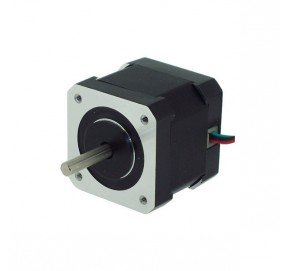
\includegraphics[width=0.49\linewidth]{\figures/photoMoteur1.jpg}
    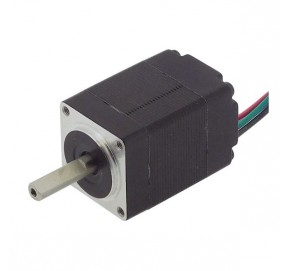
\includegraphics[width=0.49\linewidth]{\figures/photoMoteur2.jpg}
    \decoRule
    \caption[
    Moteur 17HM15-0904S et moteur S20STH30-0604A]{
    Moteur 17HM15-0904S et moteur S20STH30-0604A}
    \label{fig:Moteur 17HM15-0904S et moteur S20STH30-0604A}
    \end{figure}

Le premier a été choisi pour la rotation et l'inclinaison car il est suffisamment couple pour mouvoir le télescope et avec précision. \newline 
A l'origine, nous en avons trouvé un exemplaire sur les imprimantes 3D et nous avons vérifié s'il répondait à nos contraintes.  
Le second est plus léger que le premier, moins puissant. Il est plus adapté pour changer le zoom au bout de la flêche du télescope. Il est indispensable de limiter le poids au bout de la flêche du télescope pour faciliter des ses déplacements.   

\section{Le contrôleur}

Le contrôleur est une carte qui à partir de front montant en entrée réalise une PWM pour contrôler un moteur pas à pas.
Cette carte A4988 opto-isolée permet l’entraînement de moteur pas à pas bipolaire à micropistes Allegro A4988. Il est doté d’une protection contre les surintensités et d’une surchauffe ainsi que de cinq résolutions différentes en micropas (jusqu’à 1/16 pas). Il fonctionne de 8 V à 35 V et peut fournir jusqu’à environ 1 A par phase sans dissipateur de chaleur ni flux d’air forcé.

\begin{figure}[H]
    \centering
    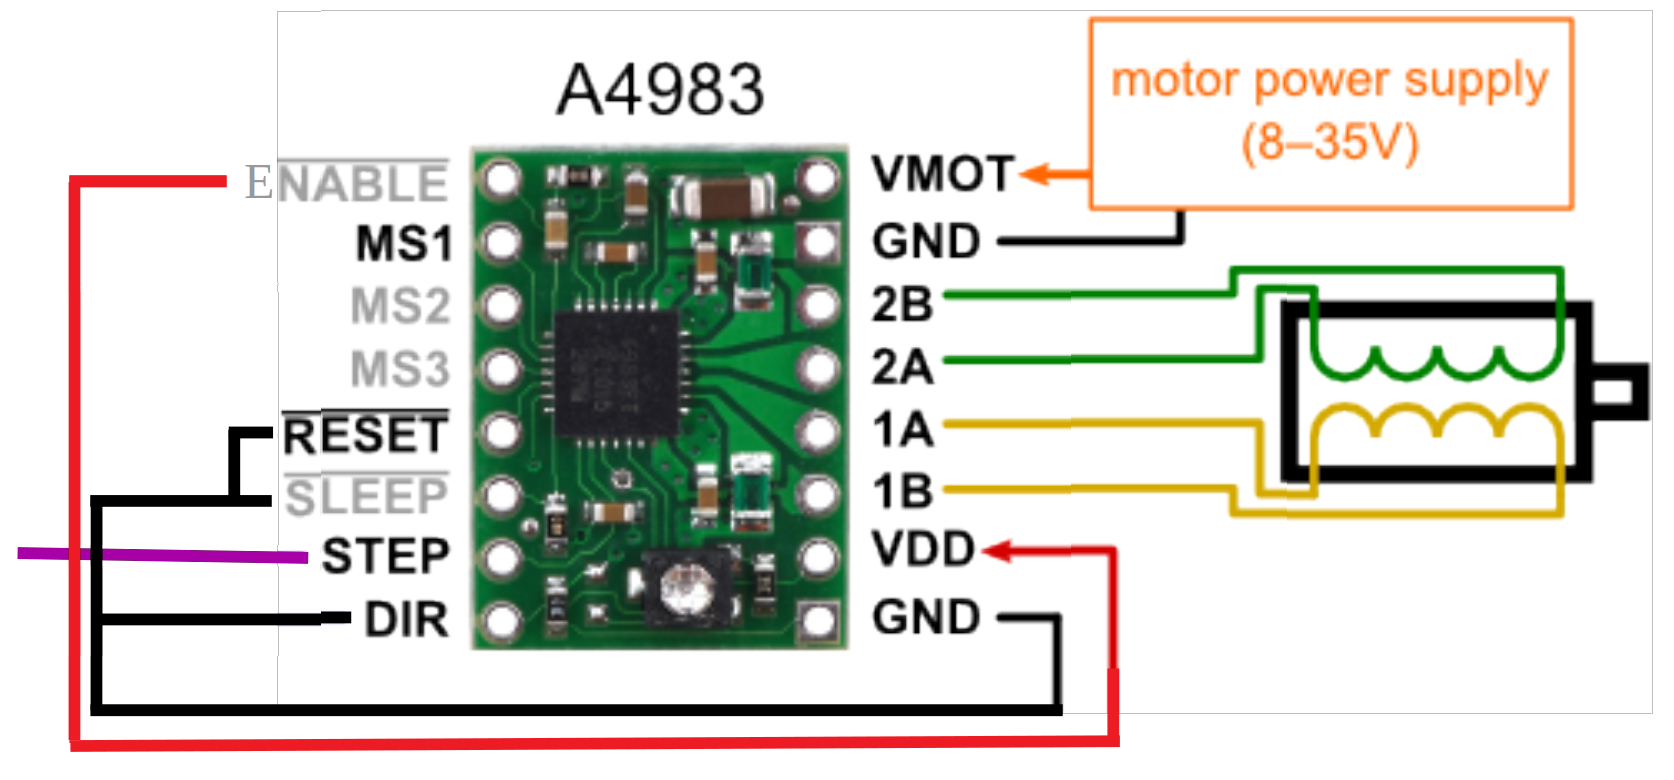
\includegraphics[width=0.6\linewidth]{\figures/sch_a4983.png}
    \decoRule
    \caption[
    Photo du contrôleur A4988]{
    Photo du contrôleur A4988}
    \label{fig:Photo du contrôleur A4988}
    \end{figure}

\section{Validation des moteurs et du câblage}
\begin{figure}[H]
    \centering
    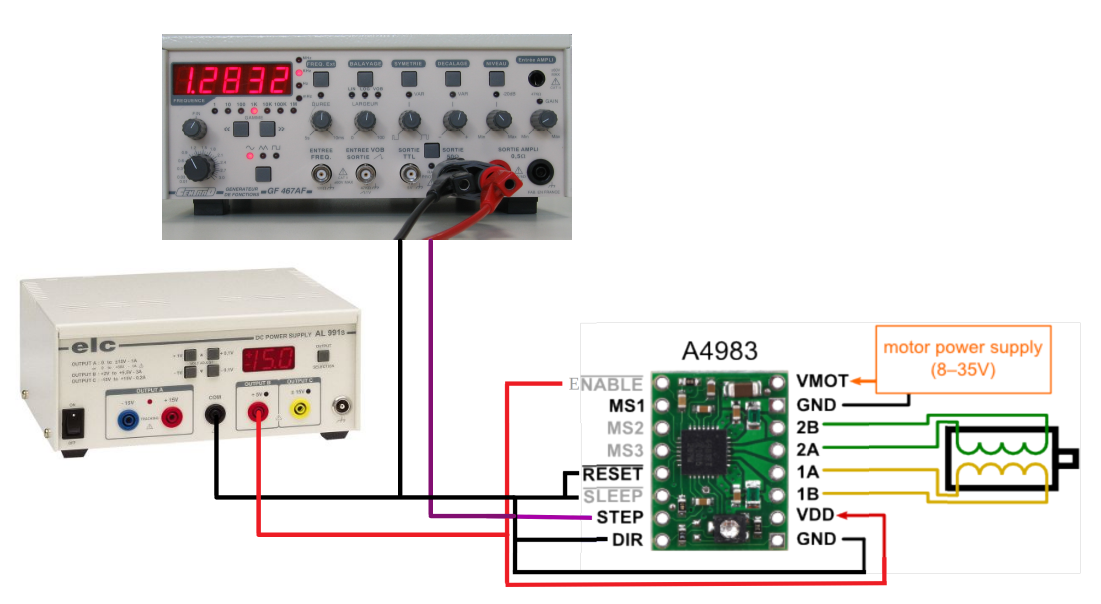
\includegraphics[width=0.8\linewidth]{\figures/sch_a4988.png}
    \decoRule
    \caption[
    Schéma de câblage d'un contrôleur moteur sur la Raspberry Pi]{
    Schéma de câblage d'un contrôleur moteur sur la Raspberry Pi}
    \label{fig:Schéma de câblage d'un contrôleur moteur sur la Raspberry Pi}
    \end{figure}

Durant ce test nous avons vérifié le bon fonctionnement du moteur et contrôleur moteur. \newline
Pour nous assurer que les moteurs de rotation et inclinaison sont suffisamment couple et résistant nous avons placé une courroie autour de l'axe du moteur et au bout de ce dernier nous avons attaché une poids de 10kg.
Ce test fut un succès et nous avons validé le choix des moteurs.

\begin{figure}[H]
    \centering
    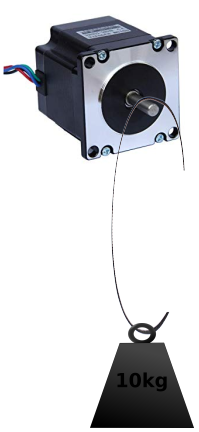
\includegraphics[width=0.3\linewidth]{\figures/test-moteur.png}
    \decoRule
    \caption[
    Test de la puissance du moteur]{
    Test de la puissance du moteur}
    \label{fig:Test de la puissance du moteur}
    \end{figure}

Nous avons profité du test pour manuellement utiliser les modes de pas en appliquant au entrées MS1, MS2, MS3 du 5 volt en suivant la documentation suivante.

\begin{figure}[H]
    \centering
    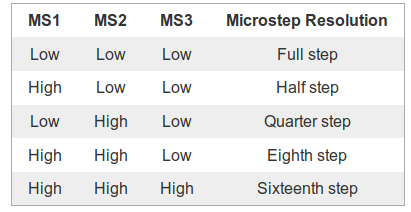
\includegraphics[width=0.5\linewidth]{\figures/doc_MS_a4988.png}
    \decoRule
    \caption[
    Documentation microStep a4988]{
    Documentation microStep a4988}
    \label{fig:Documentation microStep a4988}
    \end{figure}

\vspace{1cm}








